\documentclass[10pt, leqno]{exam}
\usepackage{xspace}
%\usepackage{listings}
%\usepackage{empheq}
%\usepackage{color}
%\usepackage{multirow}
%\usepackage{multicol,amsthm}
\usepackage{amsmath}
\usepackage{enumerate}
\usepackage{verbatim}
%\usepackage{wasysym}
\usepackage{float}
%\usepackage[pdftex]{graphicx}
\usepackage{mathtools}
%\usepackage{sidecap}
%\usepackage{wrapfig}
\usepackage{hlin}
\usepackage{jeffe}
\usepackage{boxes}
\renewcommand{\labelitemi}{--}
\renewcommand{\labelitemii}{$\bullet$}

\newcommand{\name}{Henry Lin - halin2}
\newcommand{\assignment}{Random Variables}
\renewcommand{\date}{September 24th}
\newcommand{\class}{CS 498CL1, Fall 2015}

%\setlength{\parskip}{\baselineskip}%

%\newcommand{\frownie}{=D}
%\newcommand{\smiley}{=(}
\pagestyle{headandfoot}
\firstpageheadrule
\runningheadrule
\firstpageheader{\textit{\class}}
                {\textit{\name}}
                {\textit{\date}}
\runningheader	{\textit{\class}}
                {\textit{\assignment}}
                {\textit{Page \thepage\ of \numpages}}
\firstpagefooter{}{}{}
\runningfooter{}{}{}

% Fonts and typesetting
\RequirePackage[charter]{mathdesign}
\def\sfdefault{fvs}
\def\ttdefault{fvm}
\SetMathAlphabet{\mathsf}{bold}{\encodingdefault}{\sfdefault}{b}{\updefault}
\SetMathAlphabet{\mathtt}{bold}{\encodingdefault}{\ttdefault}{b}{\updefault}
\SetMathAlphabet{\mathsf}{normal}{\encodingdefault}{\sfdefault}{\mddefault}{\updefault}
\SetMathAlphabet{\mathtt}{normal}{\encodingdefault}{\ttdefault}{\mddefault}{\updefault}
\usepackage{microtype}
\setlength\parindent{0pt}

\begin{document}

    \textbf{{\LARGE \assignment}}

    \section{Random Variables}
%%%%%%%%%%%%%%%%%%%%%%%%%%%%%%%%%%%%%%%%%%%%%%%%%%%%%%%%%%%%%%%%%%%%%%%%%%%%%%%%
    \black{
    \textbf{Definition}. A \textbf{random variable} $X$ is a function from
    the set of outcomes to the real numbers; $X : \Omega \to \RR$.
    }

    This definition is intimidating to students. Instead, think of random
    variables to be \textbf{anything} in this world that could correspond
    to something we don't know the outcome of, a priori to an observation.

    \medskip

    Examples:
    \begin{itemize}
    \item The outcome of a coin toss. (Discrete)
    \item Whether or not the cat is dead in the box with poison. (Discrete)
    \item Your possible grade in this course. (Continuous, if we consider real numbers.)
    \end{itemize}
    Once we make a valid mapping between one of these outcomes to a real number,
    we then \textit{formally} have what is called a random variable.

    \medskip

    Example. Page 128, Worked example 5.1. Let $X$ be a random variable describing
    the outcome of two consecutive coin tosses. Then we could assign the
    following outcomes to the following integers:
    \begin{itemize}
    \item TT: 0
    \item TH: 1
    \item HT: 2
    \item HH: 3
    \end{itemize}
    The book does this kind of mapping without being totally explicit about it.

    \medskip

    Random variables can either be \textbf{discrete} or \textbf{continuous}.
    The biggest difference between a discrete and continuous random variable
    is, a discrete random variable has countably many outcomes, and
    a continuous random variable has uncountably many.\footnote{A set
    $A$ is countable if it is finite, or there is a bijection between
    $A$ and the set of natural numbers $\NN$.}

    \medskip

    We will see below that distinguishing the two is important in understanding
    some probability fundamentals and notation.

    \section{Probability Distributions}

    A \textbf{probability distribution} is an assignment (function)
    between states of the random variable with a value between $[0, 1]$.
    We'll use
    $$P(X)$$
    to denote the probability distribution itself, and not values from
    the distribution.
    \begin{itemize}
    \item When $X$ is finite, the probability distribution is sometimes
    referred to as the \textbf{probability mass function} (pmf). This can
    be notated several ways, including $P(X = x)$ or $P(x)$. The book
    uses $P(\set{X = x})$.
    \item When $X$ is continuous, the probability distribution is sometimes
    referred to as the \textbf{probability density function} (pdf). This
    can be notated several ways, usually $p(x)$. (\textit{Notice the lowercase
    $p$}.)
    \end{itemize}

    Observe the analogies mathematicians tried to make when distinguishing
    these two kinds of random variables. Discrete random variables put their
    probability on specific numbers (\textit{masses}), while continuous random variables
    spread their probability along a number line like a spread of butter on bread.
    \begin{figure}[H]
    \centering
    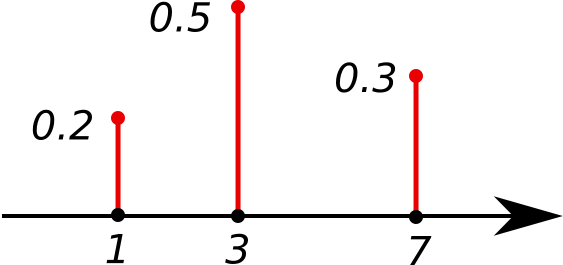
\includegraphics[scale=0.3]{discrete.png}
    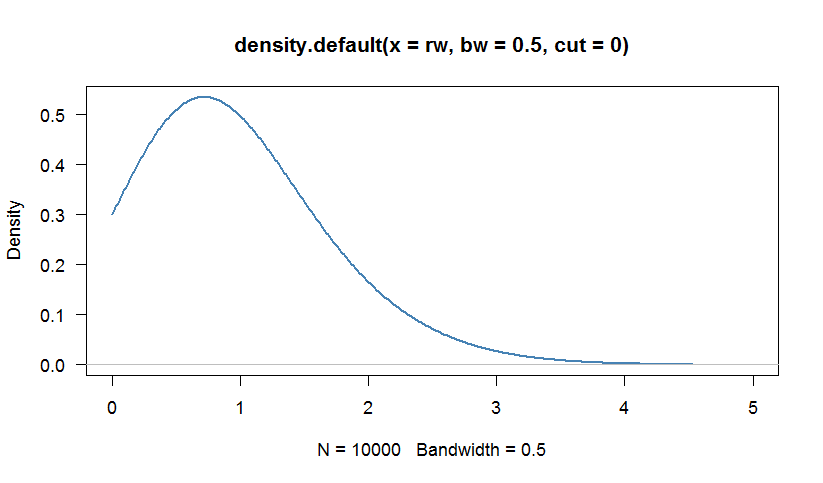
\includegraphics[scale=0.3]{continuous.png}
    \end{figure}
    The reason why continuous random variables are usually denoted as $p(x)$
    rather than $P(x)$ is because mathematicians are used to continuous functions
    being lowercase (like $f(x)$, $g(x)$, \dots); it's often the case that $p(x)$
    has a "closed" function form.

    \medskip

    For any valid probability distribution, we have
    these two properties.
    \begin{itemize}
    \item For any $x \in X$, $P(x) \geq 0$ for discrete random variables.\footnote{
    Observe the abuse of notation here with "$x \in X$". $X$ is not a set, but
    this is how mathematicians express a possible outcome from $X$.}
    $p(x) \geq 0$ for continuous random variables.
    \item $\sum_{x \in X} P(X = x) = 1$ for a discrete random variable.
    $\int_{-\infty}^{\infty} p(x) = 1$ for a continuous random variable.
    \end{itemize}

    I'll make a very important distinction here:
    \red{
        \begin{itemize}
        \item For a discrete random variable $X$, $P(X = x)$ is a valid probability.
        \item For a continuous random variable $X$, $P(X = x)$ is \textbf{not} a
        valid probability. To denote probabilities with continuous random
        variables, you need $P(a \leq X \leq b) = \int_a^b p(x)dx$.
        \footnote{Well okay. I guess in some notations you
        could use this as a placeholder for zero. But even \textit{saying} this
        in the context of continuous random variables sounds weird.}
        \end{itemize}
    }

    \section{Cumulative Distribution Functions}

    Skipped.

    \newpage

    \section{Expected Value}

    Well, what do we expect $X$ to be when we observe it? Expectation
    provides this very nice intuition.
    \newcommand{\EE}[1]{\mathbb{E}[#1]}
    \black{
        The \textbf{expected value} $\EE{X}$ of a random variable $X$ is
        given by
        \begin{itemize}
        \item $\EE{X} = \sum_{x \in X} xP(X = x)$ when $X$ is discrete
        \item $\EE{X} = \int_{-\infty}^{\infty} xp(x)$ when $X$ is continuous
        \end{itemize}
    }
    There are two intuitions to this definition.
    \begin{itemize}
    \item You expected value is equal to a \textit{weighted average} of
    each $x$. If you interpret $P(X = x)$ to be a weight, and each $x$ to be
    some kind of score, the expected value will tend to the $x$ that
    is assigned the greatest weight.
    \item The expected value is the "balancing point" on a continuous
    distribution. (If you think of a disk that isn't uniform in density
    the fulcrum of the disk is where the expected value lies.)
    \end{itemize}
    \begin{figure}[H]
    \centering
    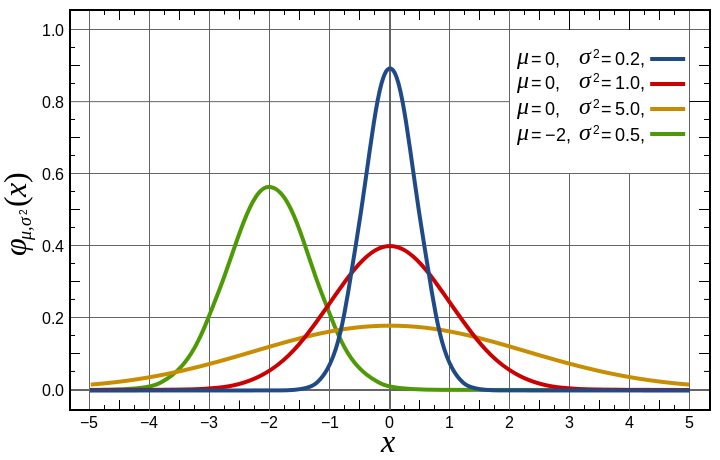
\includegraphics[scale=0.5]{expected-value.png}
    \caption{The expected value is denoted as $\mu$ in this figure.}
    \end{figure}

    \medskip

    If we interpret a dataset of exam scores, how do we expect the next
    student to do? The best guess is, probably average. This draws a
    very important point.
    \black{
        For a finite dataset $\set{x}$ of $N$ items, let us interpret $freq(x) / N$,
        the frequency of an entry over the total number of entries, to represent
        the probability of $x$, $P(X = x)$.

        \medskip

        Then $\EE{X} = \text{mean}(\set{x})$, where $\text{mean}(\set{x}) =
        \frac{1}{N}\sum_x x$.
    }


\end{document}
